\title{Predicting Pull Request Acceptance on GitHub from Social Factors}
\author{Matthew Heston}
\date{}

\documentclass[12pt]{article}
\usepackage{graphicx}
\usepackage{fixltx2e}
\usepackage{ntheorem}
\newtheorem{hyp}{Hypothesis}

\begin{document}
\maketitle

\section{Introduction}
GitHub is a social website that open source software developers use to host
their software projects and to browse other developers' projects. It includes
many features that are present on social networking sites, such as the ability
to follow other users and leave comments on projects. In the study of computer
supported cooperative work, GitHub provides a wealth of data, as it is a
centralized location where many different tasks take place. For example, users
can create bug reports, submit fixes, and engage in discussions about new
features all on one website.  In this study, we use statistical and machine
learning methods on data from GitHub repositories to explore how different
social factors may affect the acceptance of code changes from first time
contributors.

\subsection{Related Work}
GitHub itself has not been extensively studied. ~\cite{choi_herding_2013} use
data from the website to examine what they call \textit{herding behavior} of
developers in open source projects.  ~\cite{mcdonald_performance_2013} provide a
qualitative exploratory study on how developers on the website measure success
of projects. Of importance to our study is their findings that developers
believe the GitHub interface has changed the way developers are able to
participate in the community. While they describe how features of the website
are used by developers to measure community involvement and activity, we are
concerned with how these features can provide measures that insight into how
contributions by new community members are accepted by core members.

While there are not many studies on GitHub itself, there are many studies that
explore different open source communities. These include theoretical
perspectives on knowledge building and success in open source
projects~\cite{hemetsberger_learning_2006}~\cite{hemetsberger_collective_2009}
and the motivations of open source
developers~\cite{hertel_motivation_2003}\cite{lakhani_why_2003}.

Our study seeks to which factors contribute to the acceptance of code
contributions of first time contributors. We draw on findings from previous
studies that describe the joining process of new developers
~\cite{huang_mining_2005}\cite{von_krogh_community_2003}. We also draw from work
that describes joining processes not only in open source software, but also from
other computer mediated collaborative contexts, such as
Wikipedia~\cite{bryant_becoming_2005}. Our goal is to provide an empirical
understanding of community acceptance on a relatively new social platform.



\paragraph{Outline}
The remainder of this article is organized as follows.
Section~\ref{data} begins with a description of some of the terminology specific
to GitHub, since many of the features in our models rely on an understanding of
this terminology. We then describe how we measured various social factors and
present our hypotheses. In Section~\ref{methods} we describe our experiments. We
find that the variables we chose lack predictive power of pull request
acceptance. Section~\ref{discussion} describes why our models may have failed
and presents some observations from the data. Finally, Section~\ref{conclusion}
presents our conclusions and ideas for future work.

\section{Data}\label{data}

\paragraph{Terminology} A software project on the website is referred to as a
\textit{repository}. Any user on GitHub can \textit{star} a repository. Users
star repositories to be able to easily navigate to it and to receieve updates on
activity from the repository. If a developer wants to contribute to another one
of developer's repositories, he can \textit{fork} the repository, which creates
a copy of the project for him to work on. As the developer makes changes to this
code, he \textit{commits} his changes. A \textit{commit} is a snapshot of the
code at a certain point in time. When the developer is finished, he can submit a
\textit{pull request} to the owner of the project. All pull requests for a
project are viewable on GitHub, and any user of the site can comment on them. A
pull request can have a status of open or closed. A status of open indicates
that that owner of the repository has not made a decision about whether or not
to include the changes. If the owner of a repository wants to incorporate the
changes the developer made, he can \textit{merge} them into the repository. A
pull request can be closed without being merged, which means that the changes
the developer made were not accepted.

Data was collected using the GitHub API.\footnote{http://developer.github.com/}
We collected pull requests from 45 different repositories. The repositories
selected came from the top 100 most starred repositories on GitHub. We chose
popular repositories with the assumption that they would be maintained by an
active community. We only consider pull requests with a status of closed. This
resulted in approximately 44,400 pull requests. We then filter this data set to
include only the first pull request a user submitted, which results in 13,383
pull requests. Of these, 4,352, or 32.5\% of the pull requests were merged. We
consider several features, both on the pull request itself as well as the
repository.

\subsection{User Participation}
In their study on members of Wikipedia, ~\cite{bryant_becoming_2005} note that
members initially become involved through peripheral activities. These are
simple and low risk activities members can take part in to learn more about the
community before trying to become major contributors. Similarly,
~\cite{von_krogh_community_2003} from observing open source communities generate
the construct of a \textit{joining script}, where each project has a set of
tasks for new developers to go through before being accepted into the community.
In the case of GitHub, we consider the act of commenting on previous pull
requests to be the main peripheral activity a user can participate in before
submitting a pull request of their own. For each pull request in our data set,
we then count the number of previous pull request discussions the user
participated in before submitting their own pull request, and present our first
hypothesis.

\begin{hyp}
Community members who have been active in previous discussions are more likely
to have their code changes accepted.
\end{hyp}

\subsection{Reputation of User}
In addition to participation within the community, we also suspect that a
developer's reputation can affect whether or not his pull request is accepted.
In particular, we hypothesize that a user who has popular projects of his own is
more likely have his pull requests accepted. To measure this property, we use
the total number of stars a user's repositories has received. This seems to be a
good proxy for measuring the popularity of projects. Unfortunately, we cannot
retrieve historical data for stars from the GitHub API. It is therefore not
possible to know how many stars a user's projects had at the time he submitted
his pull request. We do, however, know the when repositories were created.
Therefore, to measure a user's reputation, we look at repositories that were
created at the time his pull request was submitted, and sum the current number
of stars those projects have at the time our data was collected. This is not a
perfect approximation, as some of these projects may have gained many more stars
long after the pull request was submitted. However, since we cannot access
historical data, we rely on this as an approximation for user reputation.

\begin{hyp}
Community members who have other popular projects are more likely to have their
code changes accepted.
\end{hyp}

\subsection{Attention Pull Request Recieves}
We consider the attention the pull request receives, which we measure as the
total number of comments on the pull request. Our intuition is that a high
number of comments indicates the pull request is generating interest within the
community and is therefore more likely to be merged.

\begin{hyp}
Pull requests with a high number of comments are more likely to be accepted.
\end{hyp}

\subsection{Number of Other Contributors}
~\cite{viegas_studying_2004} find what they call a \textit{first-mover
advantage} in the editing of Wikipedia articles, wherein the first contribution
to a page tends to survive longer and recieve less modifications than following
contributions. They hypothesize that the first user sets the tone of the article
and their contributions therefore are more likely to survive. We predict a
similar effect in pull requests, where the first persons to submit pull requests
are more likely to be accepted.

\begin{hyp}
The likelihood a pull request is accepted declines as the number of contributors
to a repository increases.
\end{hyp}

\subsection{Number of Previous Commits}
Similar to the above hypothesis, we also measure the number of commits that have
occurred in a repository prior the submission of the pull request. In addition
to counting the number of previous contributors, we believe that commits here
can be used as an estimate of how much activity has taken place in a codebase,
and that as more activity occurs and project complexity grows, the likelihood of
a pull request being accepted decreases.

\begin{hyp}
The likelihood a pull request is accepted declines as the number of commits to a
repository increases.
\end{hyp}

\subsection{Size of the Pull Request}
We use two metrics to measure the size of the commit, both the number of commits
and the number of changes. As mentioned previously, a commit is a snapshot of
the code at a certain point in time. Different developers might have different
commit habits, but in general, larger changes will probably include more
commits. The number of changes is calculated simply as the number of lines added
and the number of lines deleted. As an example to help differentiate these two
metrics, imagine the scenario of changing the name of a widely used variable
across the code base. Every line where this variable name appears would be
treated as being deleted and re-added using the new variable name by git,
resulting in a large number of changes. The developer, however, would likely
only make one commit to capture this change. We predict that smaller pull
requests are more likely to be accepted, since they can be reviewed quickly and
are unlikely to introduce new complexity.

\begin{hyp}
The likelihood a pull request is accepted declines as the size of the pull
request increases.
\end{hyp}

\section{Methods}\label{methods}
To test the relationship between the variables identified in Section~\ref{data},
we apply a logistic regression model using these variables as indepedent
variables and the binary outcome of merged or not as the dependent variable. We
create categorical independent variables by binning the data. The results from
the regression are shown in Table~\ref{logit}. In general, we do see the
correlations we expect in the model, with the exception of the number of
comments that the pull request receives, where we see a negative correlation. 

Examining the decrease in deviance from the null deviance from our parameters
indicates our model significantly ourperforms a null model. However, the
$\chi^{2}$ value for the residual deviance is approximately equal to 1,
indicating that the logit model overall may be a poor fit.


\begin{table}[!htbp] \tiny \centering 
\caption{Logistic Regression Results} 
\label{logit} 
\begin{tabular}{@{\extracolsep{5pt}}lc} 
\\[-1.8ex]\hline 
\hline \\[-1.8ex] 
& \multicolumn{1}{c}{\textit{Dependent variable:}} \\ 
\cline{2-2} 
\\[-1.8ex] & merged \\ 
\hline \\[-1.8ex] 
User participation\textsubscript{1} & 0.242 \\ 
& (0.421) \\ 
& \\ 
User participation\textsubscript{2} & 0.912$^{*}$ \\ 
& (0.513) \\ 
& \\ 
User participation\textsubscript{3} & 1.729$^{***}$ \\ 
& (0.617) \\ 
& \\ 
Attention pull request receives\textsubscript{1} & $-$0.795$^{***}$
\\ 
& (0.155) \\ 
& \\ 
Attention pull request receives\textsubscript{2} & $-$0.053 \\ 
& (0.325) \\ 
& \\ 
Attention pull request receives\textsubscript{3} & $-$0.019
\\ 
& (0.524) \\ 
& \\ 
User reputation\textsubscript{1} & 0.185$^{*}$
\\ 
& (0.101) \\ 
& \\ 
User reputation\textsubscript{2} &
0.192 \\ 
& (0.130) \\ 
& \\ 
User reputation\textsubscript{3}
& 0.342$^{**}$ \\ 
& (0.143) \\ 
& \\ 
Number of commits\textsubscript{1}
& $-$1.195$^{***}$ \\ 
& (0.416) \\ 
& \\ 
Number of commits\textsubscript{2}
& $-$3.218$^{***}$ \\ 
& (1.013) \\ 
& \\ 
Number of commits\textsubscript{3}
& $-$13.219 \\ 
& (114.104) \\ 
& \\ 
Number of changes\textsubscript{1}
&
$-$0.221$^{**}$
\\ 
& (0.108) \\ 
& \\ 
Number of changes\textsubscript{2}
&
$-$0.609$^{***}$
\\ 
&
(0.148)
\\ 
& \\ 
Number of changes\textsubscript{3}
&
$-$0.620$^{***}$
\\ 
&
(0.192)
\\ 
&
\\ 
Number of repository commits\textsubscript{1}
&
$-$0.306$^{***}$
\\ 
&
(0.050)
\\ 
&
\\ 
Number of repository commits\textsubscript{2}
&
$-$0.037
\\ 
&
(0.060)
\\ 
&
\\ 
Number of repository commits\textsubscript{3}
&
0.245$^{***}$
\\ 
&
(0.085)
\\ 
&
\\ 
Number of contributors\textsubscript{1}
&
$-$0.103$^{*}$
\\ 
&
(0.055)
\\ 
&
\\ 
Number of contributors\textsubscript{2}
&
$-$0.657$^{***}$
\\ 
&
(0.098)
\\ 
&
\\ 
Number of contributors\textsubscript{3}
&
$-$0.526$^{***}$
\\ 
&
(0.140)
\\ 
&
\\ 
Constant
&
$-$0.547$^{***}$
\\ 
&
(0.031)
\\ 
&
\\ 
\hline
\\[-1.8ex] 
Observations
&
13,383
\\ 
Log
Likelihood
&
$-$8,282.562
\\ 
Akaike
Inf.
Crit.
&
16,609.120
\\ 
\hline 
\hline
\\[-1.8ex] 
\textit{Note:}
&
\multicolumn{1}{r}{$^{*}$p$<$0.1;
$^{**}$p$<$0.05;
$^{***}$p$<$0.01}
\\ 
\normalsize 
\end{tabular} 
\end{table} 

\section{Discussion}\label{discussion}
Visualizing some variables demonstrates that they may be a poor choice in
attemping to distinguish between merged and not merged pull requests. In
Figure~\ref{social_plot}, we see a scatter plot of user activity and the number
of comments on pull requests for both merged and not merged pull requests. In
both cases, most of the values for these features are zero. This in itself is an
interesting observation. In evaluating the types of activity which take place in
developer joining scripts, ~\cite{von_krogh_community_2003} note that the most
common type of activity is to join an ongoing technical discussion, rather than
suggest a technical solution. In a discussion of successful developers on the
Python project, ~\cite{ducheneaut_socialization_2005} describe the first steps
of their trajectory as including peripheral monitoring of development activity
and reporting of bugs. In both cases, developers first participate in peripheral
activities. Both of these studies examine CVS repositories and project mailing
lists. The GitHub interface makes it relatively easy for a user to fork a
repository, make changes, and submit the changes for consideration. Previous
studies on GitHub have shown that the number of contributions did increase for
some projects that moved from other hosting options to
GitHub~\cite{mcdonald_performance_2013}. It is possible this interface lowers
the barrier of entry for a developer who wants to contribute to a project. It is
also interesting to compare this to Figure~\red{social_plot_repeaters}, which
shows the same data, but only for those users who later submit another pull
request. The goal here is to filter out users who may be submitting a one off
big fix, and focus on users who are interested in becoming members of the
community by continuing to submit more changes over time. We see a similar
effect in the scatter plot, however, indicating that even users who will
continue to contribute multiple pull requests do not necessarily participate
before submitting, and that there is not much differentiation in these variables
between those pull requests that get merged and those that do not.

\begin{figure}[p] \centering
\caption{Visualization of number of comments on a pull request and user
participation variables. Merged pull requests are blue. Not merged are red.}
\label{social_plot}
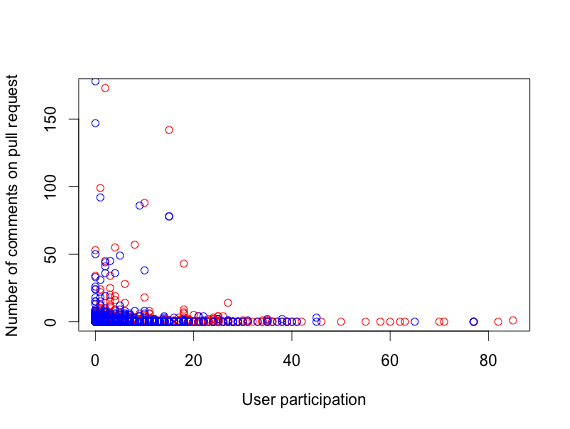
\includegraphics[scale=0.75]{figures/social_variables.png}
\end{figure}

\begin{figure}[p] \centering
\caption{Visualization of number of comments on a pull request and user
participation variables for pull requests by users who later submitted at least
one more pull request. Merged pull requests are blue. Not merged are red.}
\label{social_plot_repeaters}
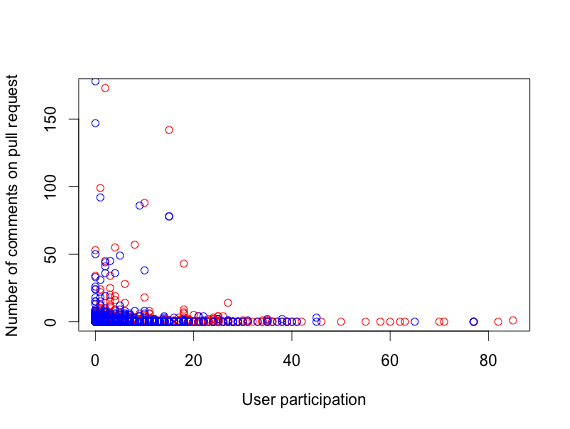
\includegraphics[scale=0.75]{figures/social_variables.png}
\end{figure}

Another interesting observation is the negative relationship between the number
of comments on a pull request and the likelihood of it being merged. Manual
inspection of some of these pull requests suggests there are several causes for
this. For example, it may be the case that the owner of a repository is not
interested in merging a change, but other community members think the change is
valuable, so they leave comments on the pull request to encourage the repository
owner to merge it. In other cases, a discussion might develop between only the
person who submitted the pull request and the repository owner where the two of
them debate the value of the submitted change. It would be interesting to see if
inclusion of things like number of people who commented on a pull request and
analysis of linguistic features along with the number of comments on the pull
request help make it more predictive.

\bibliographystyle{plain}
\bibliography{Master}

\end{document}
